\documentclass{article}

\usepackage[T1]{fontenc}
\usepackage[utf8]{inputenc}
\usepackage[brazilian]{babel}
\usepackage{graphicx}
\usepackage[export]{adjustbox}[2011/08/13]
\usepackage{float}
\usepackage[pdftex]{hyperref}
\usepackage{epstopdf}
\usepackage{etoolbox}
\usepackage{amsmath}
\usepackage{amsfonts}
\usepackage{amssymb}
\usepackage{caption}
\usepackage{subcaption}
\usepackage{setspace}
\usepackage{tikz}
\usepackage{listings}
\usepackage{xcolor} 

\bibliographystyle{eric}
\patchcmd{\thebibliography}{\section*}{\section}{}{}


\newcommand{\R}{\ensuremath{\mathbb{R}}}
\newcommand{\Prob}{\ensuremath{\mathbb{P}}}
\newcommand{\K}{\ensuremath{\mathbb{K}}}
\newcommand{\U}{\ensuremath{\mathbb{U}}}
\newcommand{\N}{\ensuremath{\mathbb{N}}}
\newcommand{\Lg}{\ensuremath{\mathbb{L}}}
\newcommand{\T}{\ensuremath{\rm Tr}}
\newcommand{\sg}{{\sigma(x_k)}}

\newcommand{\G}{\ensuremath{\mathcal{G}}}
\newcommand{\F}{\ensuremath{\mathcal{F}}}
\newcommand{\C}{\ensuremath{\mathcal{C}}}
\newcommand{\E}{\ensuremath{\mathcal{E}}}
\newcommand{\Hn}{\ensuremath{\mathcal{H}}}
\newcommand{\Hoo}{\ensuremath{\mathcal{H}_\infty}}
\newcommand{\Hop}{\ensuremath{\mathcal{H}_{op}}}
% --------------------------------------------------
\newtheorem{theo}{Teorema}
\newtheorem{exa}{Exemplo}
\newtheorem{lemm}{Lema}
\newtheorem{coro}{Corolário}
\newtheorem{defn}{Definição}[section]

\begin{document}

\begin{titlepage}
\begin{center}

\newcommand{\HRule}{\rule{\linewidth}{0.5mm}}
% Upper part of the page. The '~' is needed because \\
% only works if a paragraph has started.

\includegraphics[width=0.15\textwidth]{logoUnicamp}~\\[1cm]

\textsc{\LARGE Universidade Estadual de Campinas}\\[1.5cm]

\textsc{\Large Faculdade de Engenharia Mecânica}\\[0.5cm]

% Title
\HRule \\[0.4cm]
{ \huge \bfseries ES664 - Laboratório de Eletrônica para Automação Industrial\\ \vspace{1cm} Relatório - Experimento 4\\
\Large{Acionamento de motor DC} \\[0.4cm] }

\HRule \\[1.5cm]

% Author and supervisor
\begin{minipage}{0.6\textwidth}
\begin{flushleft} \large
\emph{Nome:}\\
Daniel Dello Russo Oliveira\\Marcelli Tiemi Kian
\end{flushleft}
\end{minipage}
\begin{minipage}{0.2\textwidth}
\begin{flushright} \large
\emph{RA}\\ 101918\\117892
\end{flushright}
\end{minipage}

\vfill

% Bottom of the page
{\large \today}

\end{center}
\end{titlepage}


\onehalfspacing
\section{Objetivos}
	Esse relatório tem como objetivo o estudo de retificadores controlados. Analisaremos o efeito do ângulo de disparo e de cargas indutivas na saída de um retificador monofásico controlado.
	 
\section{Carga R}
Implementamos o retificador monofásico totalmente controlado detalhado no roteiro conforme mostrado na figura \ref{fig:resq} com uma lâmpada de resistência $R$ = $9.42 \Omega$.
\begin{figure}[H]
	\centering
	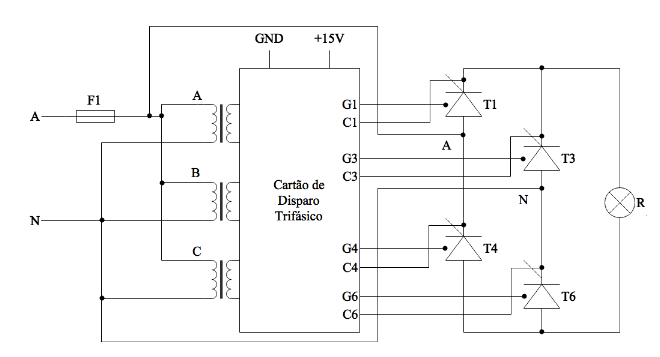
\includegraphics[width=\linewidth]{dados/resq}
	\caption{Diagrama para montagem do retificador monofásico de onda completa totalmente controlado}
	\label{fig:resq}
\end{figure}

Extraímos a curva de tensão na carga (figura \ref{fig:rvo}) e a tensão nos tiristores 3 (figura \ref{fig:rvt3}) e 6 (figura \ref{fig:rvt6}) para um ângulo de disparo $\alpha\ =\ 60^\circ$.
\begin{figure}[H]
	\centering
	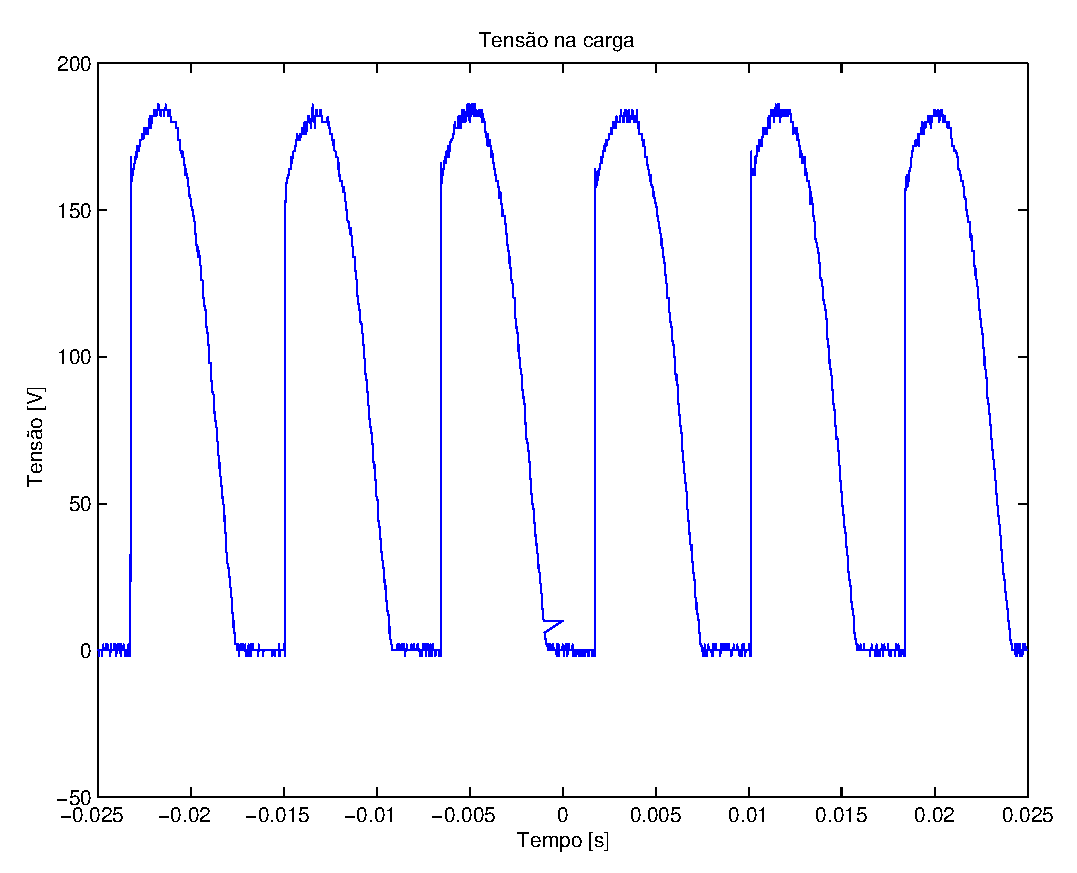
\includegraphics[width=0.7\linewidth]{dados/R/r_vo}
	\caption{Tensão na carga para retificador monofásico com carga R}
	\label{fig:rvo}
\end{figure}
\begin{figure}[H]
	\centering
	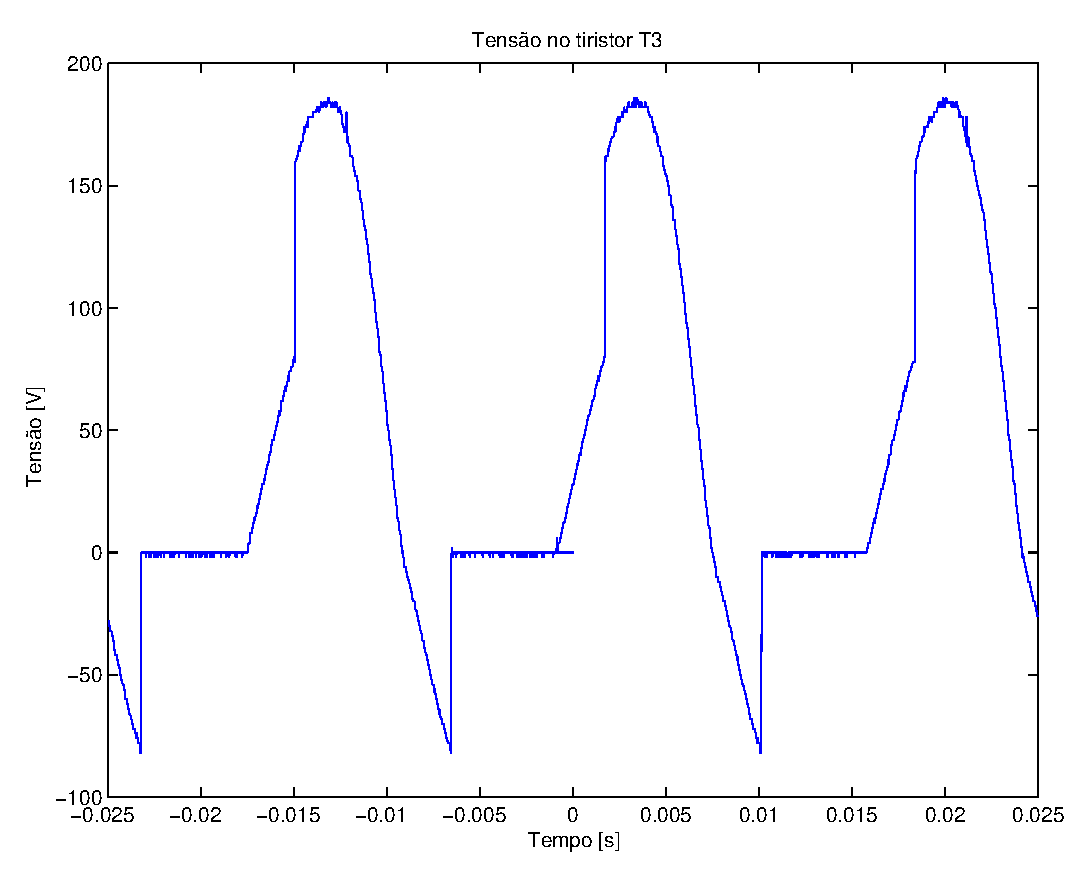
\includegraphics[width=0.7\linewidth]{dados/R/r_vt3}
	\caption{Tensão no tiristor 3 para retificador monofásico com carga R}
	\label{fig:rvt3}
\end{figure}
\begin{figure}[H]
	\centering
	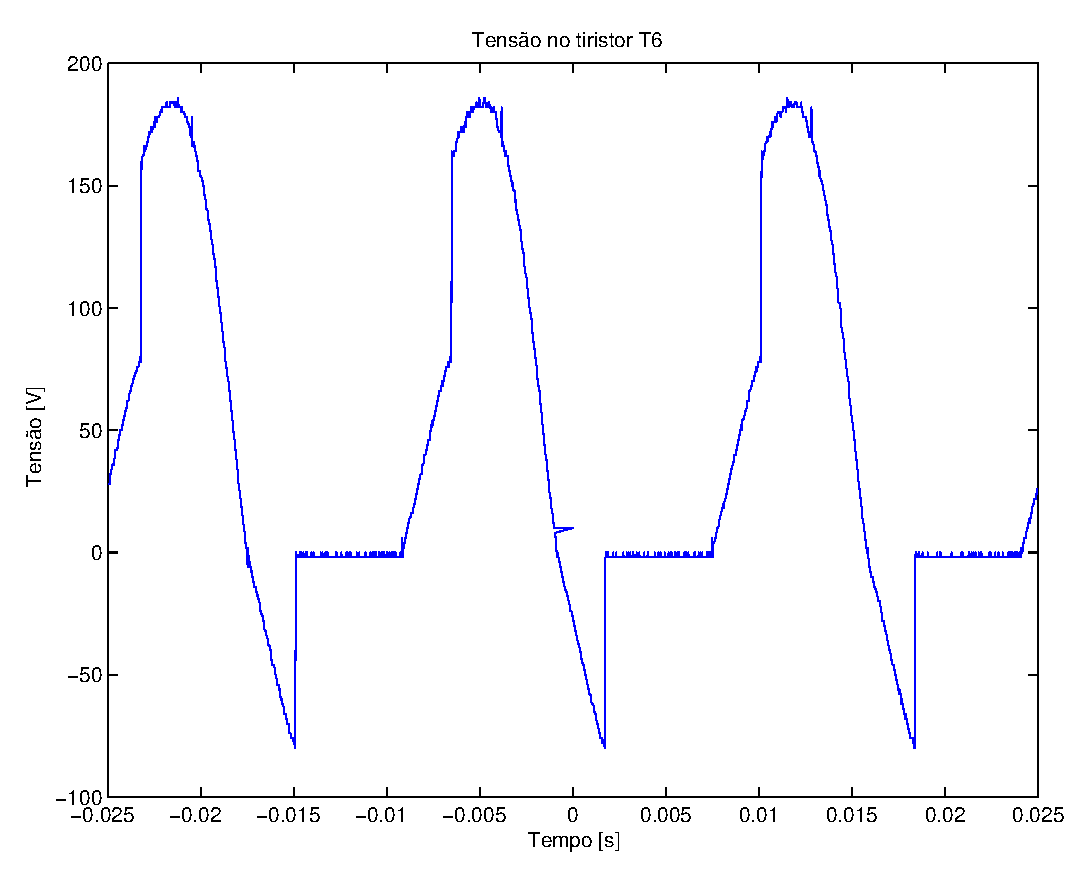
\includegraphics[width=0.7\linewidth]{dados/R/r_vt6}
	\caption{Tensão no tiristor 6 para retificador monofásico com carga R}
	\label{fig:rvt6}
\end{figure}

Medimos a tensão média e efetiva na carga, obtendo os seguintes valores:
\begin{equation}
\overline{Vo} = 93.7\ V
\end{equation}
\begin{equation}
Vo_{rms} =  121\ V
\end{equation}

Podemos calcular a tensão média teórica sobre a carga através da equação \ref{eq:rmean}
\begin{equation}
	\overline{Vr} = \frac{1}{\pi} \int_{\alpha}^{\pi}{Vs sin(\theta)d\theta} = \frac{Vs (1 + cos(\alpha))}{\pi}
	\label{eq:rmean}
\end{equation}
Para calcular o valor efetivo da tensão sobre a carga utilizamos a equação \ref{eq:rrms}.
\begin{equation}
	Vr_{rms} = \sqrt{\frac{1}{\pi} \int_{\alpha}^{\pi}{(Vs sin(\theta))^2 d\theta}} = \frac{Vs \sqrt{\pi + \frac{sin(2\alpha)}{2}- \alpha }}{\sqrt{2 \pi}} 
	\label{eq:rrms}
\end{equation}
Varrendo o ângulo de disparo $\alpha$ entre $0^\circ$ e $180^\circ$ comparamos os valores teóricos e medidos para a tensão sobre a carga, figura \ref{fig:ralpha}.
\begin{figure}[H]
	\centering
	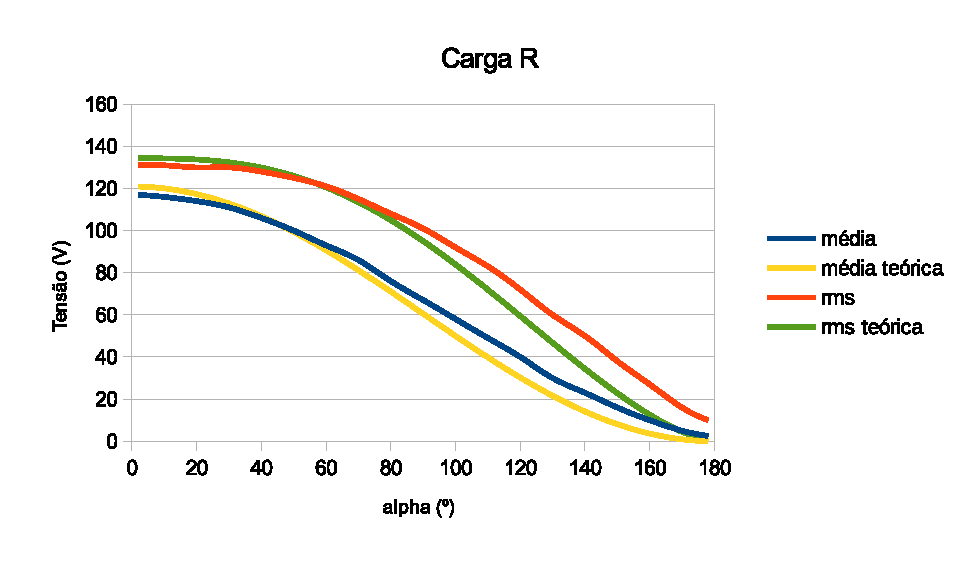
\includegraphics[width=0.7\linewidth]{dados/R/r_alpha}
	\caption{Tensão na carga média e efetiva em função do ângulo de disparo}
	\label{fig:ralpha}
\end{figure}

Como podemos ver os valores obtidos diferem pouco dos que os esperados teoricamente, as pequenas variações se devem às imprecisões de medida, à queda de tensão introduzida pelos diodos, aos componentes não ideais, entre outros fatores.

\section{Carga RL}
Conectamos então um indutor ($L$ = $43.9\ mH$) em série com o resistor mostrado na figura \ref{fig:resq}. Extraímos as curvas de tensão no resistor (figura \ref{fig:rlvr}) no indutor (figura \ref{fig:rlvl}) e na carga RL como um todo (figura \ref{fig:rlvrl}) para um ângulo de disparo $\alpha\ =\ 60^\circ$.
\begin{figure}[H]
	\centering
	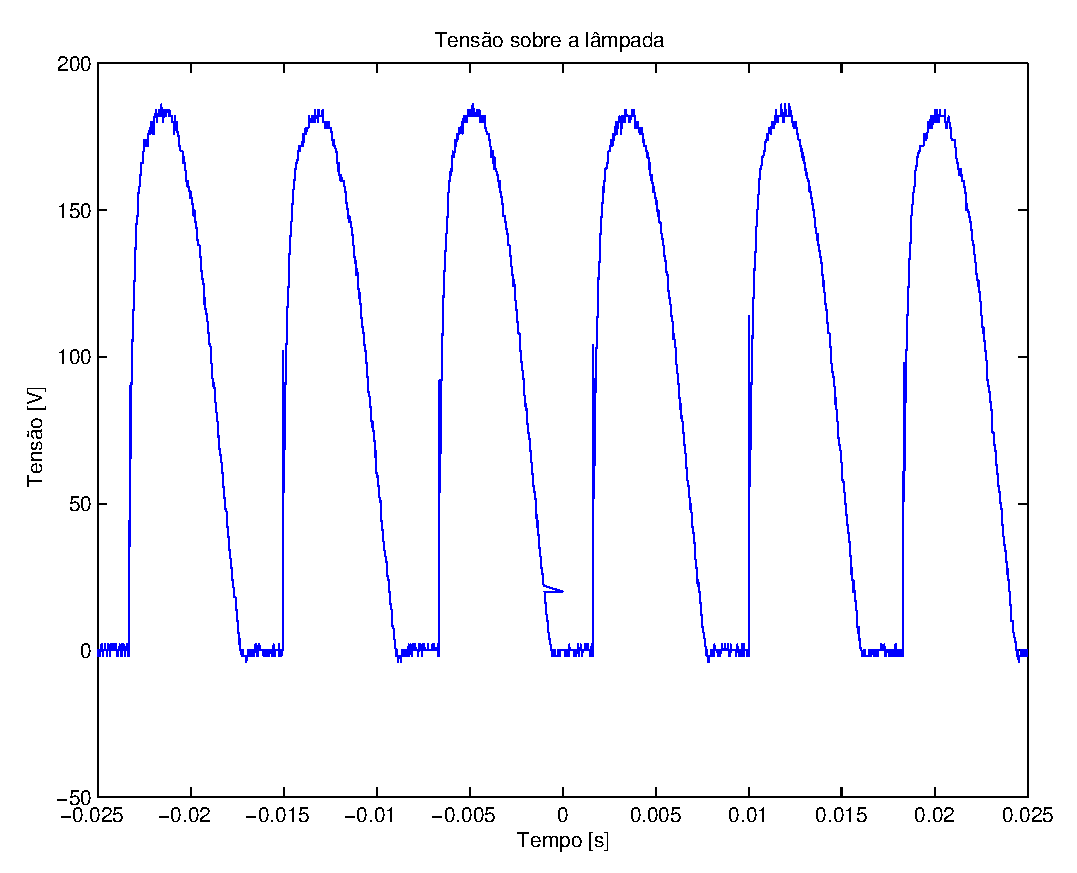
\includegraphics[width=0.7\linewidth]{dados/RL/rl_vr}
	\caption{Tensão no resistor para retificador monofásico com carga RL}
	\label{fig:rlvr}
\end{figure}
\begin{figure}[H]
	\centering
	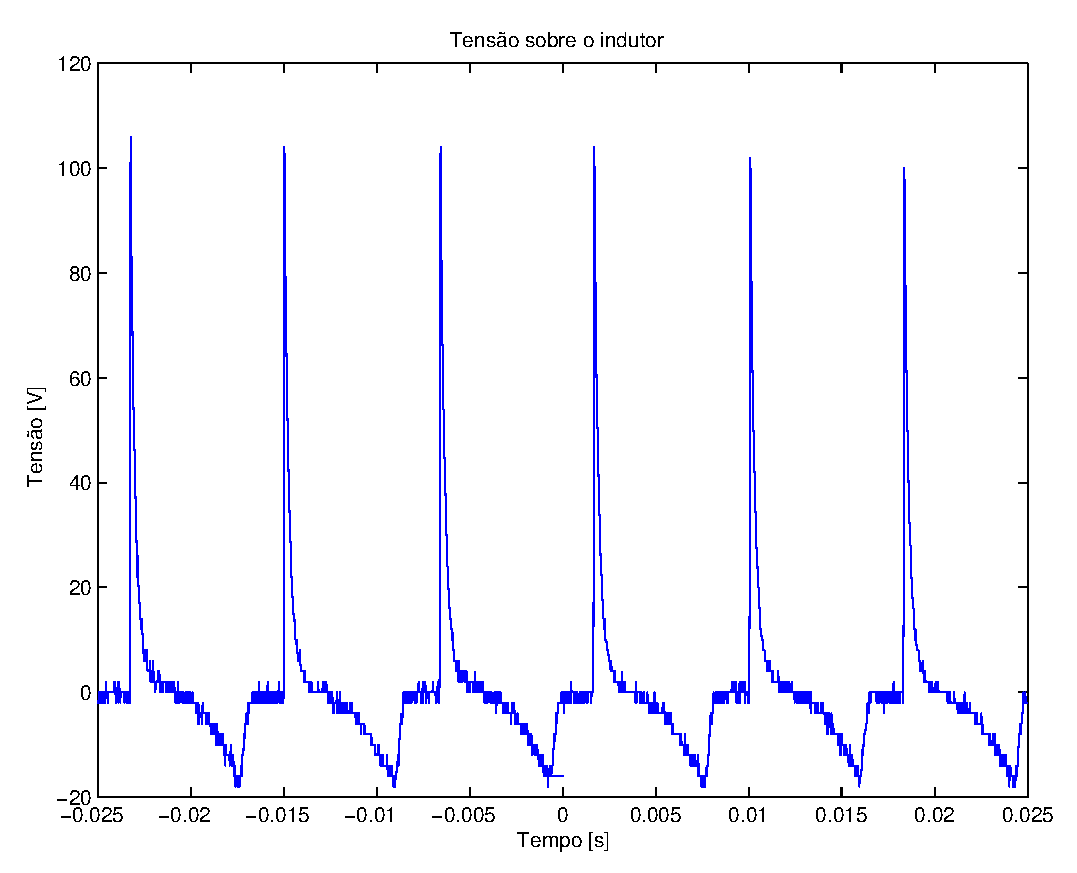
\includegraphics[width=0.7\linewidth]{dados/RL/r_vl}
	\caption{Tensão no indutor para retificador monofásico com carga RL}
	\label{fig:rlvl}
\end{figure}
\begin{figure}[H]
	\centering
	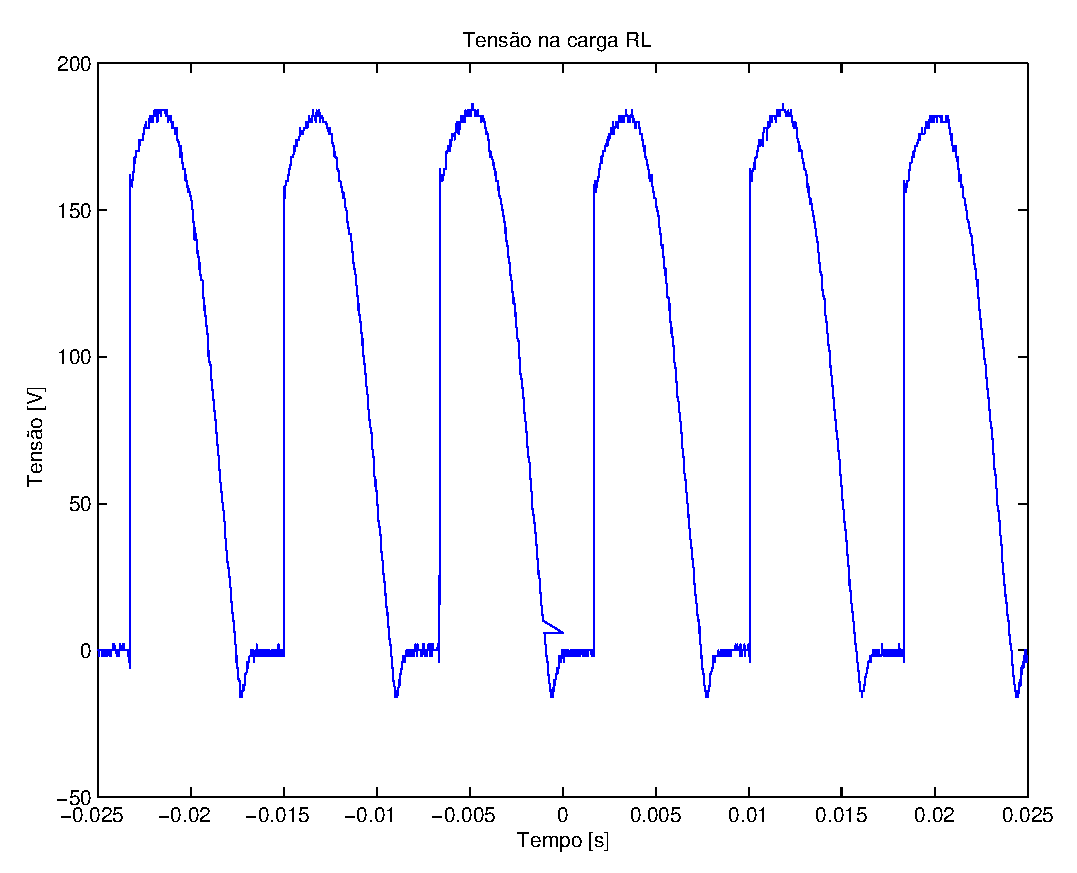
\includegraphics[width=0.7\linewidth]{dados/RL/r_vrl}
	\caption{Tensão na carga para retificador monofásico com carga RL}
	\label{fig:rlvrl}
\end{figure}
Medimos as tensões médias e efetivas na resistência R, no indutor L e na carga como um todo, obtendo os seguintes valores:
\begin{equation}
\overline{V_r} = 92\ V
\end{equation}
\begin{equation}
V_{r_{rms}} =  118\ V
\end{equation}
\begin{equation}
\overline{V_l} = 0.04\ V
\end{equation}
\begin{equation}
V_{l_{rms}} =  15\ V
\end{equation}
\begin{equation}
\overline{V_{rl}} = 93.7\ V
\end{equation}
\begin{equation}
V_{{rl}_{rms}} =  121\ V
\end{equation}

Sendo $\phi$ a defasagem introduzida pela carga indutiva:
\begin{equation}
	\phi = \arctan{(\frac{L\omega}{R})}
\end{equation}
Sabemos que a corrente sobre a carga será da forma durante o intervalo que existe condução:
\begin{equation}
	i(\omega t) = \frac{V_s}{Z}(\sin(\omega t - \phi)) - \sin(\alpha - \phi)e^{\frac{R}{L}(t - \frac{\alpha}{\omega})}
\end{equation}
Supondo um ângulo de extinção $\gamma$ teremos:
\begin{equation}
i(\pi + \gamma) = 0 = \frac{V_s}{Z}(\sin(\pi + \gamma - \phi)) - \sin(\alpha - \phi)e^{-\frac{R}{L}(\frac{\pi + \gamma - \alpha}{\omega})}
\end{equation}
Logo:
\begin{equation}
 0 = \sin(\pi + \gamma - \phi) - \sin(\alpha - \phi)e^{-\frac{\pi + \gamma - \alpha}{\tan(\phi)}}
 \label{eq:gamma}
\end{equation}
Podemos calcular a tensão média teórica sobre a carga através da equação \ref{eq:rlmean}
\begin{equation}
\overline{Vr} = \frac{1}{\pi} \int_{\alpha}^{\pi + min(\alpha, \gamma)}{Vs \sin{(\theta)}d\theta} = \frac{Vs (-\cos{(\pi + min(\alpha, \gamma))} + \cos{(\alpha}))}{\pi}
\label{eq:rlmean}
\end{equation}
Para calcular o valor efetivo da tensão sobre a carga utilizamos a equação \ref{eq:rlrms}.
\begin{equation}
Vr_{rms} = \sqrt{\frac{1}{\pi} \int_{\alpha}^{\pi + min(\alpha, \gamma)}{(Vs \sin(\theta))^2 d\theta}}
\end{equation}
\begin{equation}
Vr_{rms} = \frac{Vs \sqrt{\pi + min(\alpha, \gamma) + \frac{sin(2\alpha)}{2} - \frac{sin(2(\pi + min(\alpha, \gamma)))}{2} - \alpha }}{\sqrt{2 \pi}} 
\label{eq:rlrms}
\end{equation}

Variamos o ângulo $\alpha$ entre $0$ e $180^\circ$ e comparamos os valores teóricos e medidos para a tensão sobre a carga, figura \ref{fig:rlalpha}.
\begin{figure}[H]
	\centering
	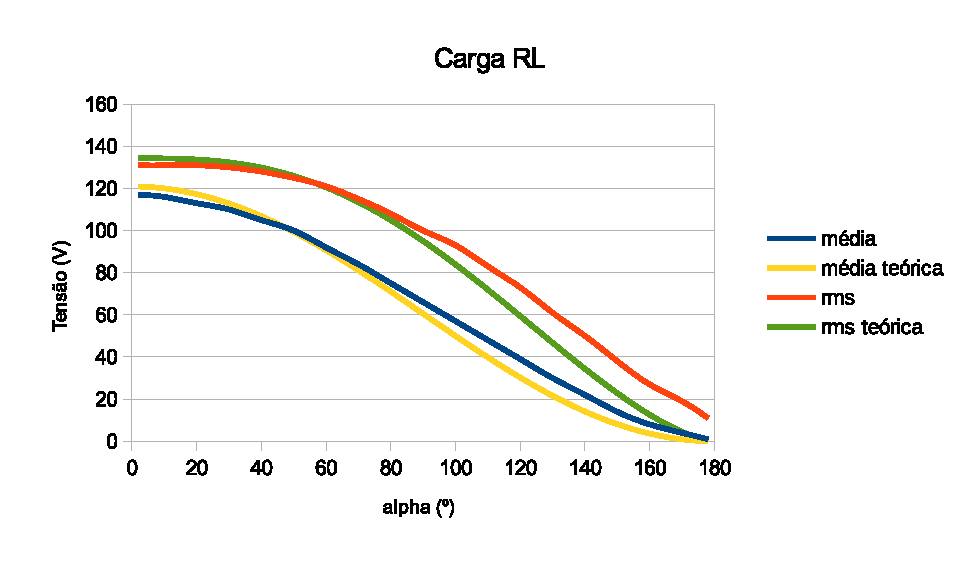
\includegraphics[width=0.7\linewidth]{dados/RL/rl_alpha}
	\caption{Tensão na carga média e efetiva em função do ângulo de disparo}
	\label{fig:rlalpha}
\end{figure}
Como podemos ver os valores medidos e teóricos pouco se assemelham. Acreditamos que um dos principais fatores causadores dessa discrepância foi a medição da resistência da lâmpada (que apresentou um valor muito menor do que o esperado e estava flutuando significativamente entre cada medida). Também precisamos levar em consideração o fato que ignoramos a resistência associada com o indutor (que não é necessariamente desprezível). Ajustamos nossa curva teóricas para uma lâmpada de $57 \Omega$ (valor medido no experimento 1) e obtivemos resultados bem mais próximos (figura \ref{fig:rlalpha57})
\begin{figure}[H]
	\centering
	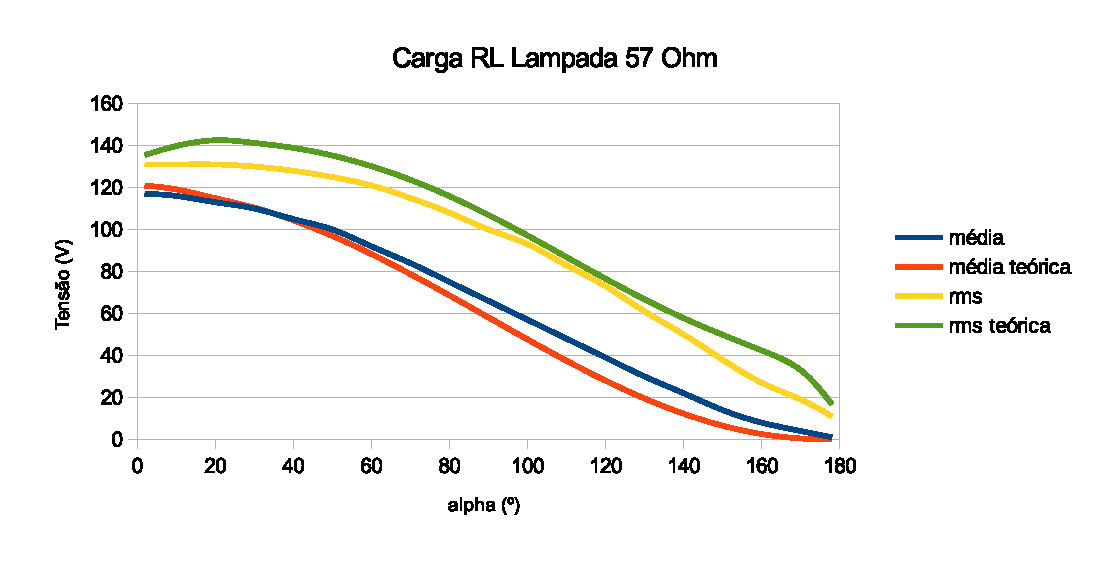
\includegraphics[width=0.7\linewidth]{dados/RL/rl_alpha57Ohm}
	\caption{Tensão na carga média e efetiva em função do ângulo de disparo para lâmpada de $57 \Omega$}
	\label{fig:rlalpha57}
\end{figure}

Calculamos o ângulo de extinção $\gamma$ teórico (para cada valor de resistência) para um $\alpha$ = $90^\circ$ resolvendo numericamente a equação \ref{eq:gamma}.
\begin{equation}
	\gamma_t = 168.15^\circ
\end{equation}
\begin{equation}
\gamma_{t_{57}} = 50.57^\circ
\end{equation}
Podemos também estimar esse valor com a tensão média medida e a equação \ref{eq:rlmean}.
\begin{equation}
	\gamma = 66.12^\circ
\end{equation}
Como podemos ver esse valor se aproxima muito mais do valor esperado para uma resistência de $57 \Omega$ do que para o valor da resistência medido.

Podemos encontrar o $\alpha_c$ para que o circuito opere no limiar entre condução contínua e descontínua utilizando a equação \ref{eq:gamma} com a condição $\gamma = \alpha_c$. Encontramos então (para cada valor de resistência):
\begin{equation}
\alpha_{ct} = 60.35^\circ
\end{equation}
\begin{equation}
\alpha_{{ct}_{57}} = 16.19^\circ
\end{equation}
%TODO FAZER SENTIDO DISSO

De acordo com a nota de aplicação do AN1048/D da ON Semiconductor, os circuitos "snubber" montado em paralelo com os tiristores como no kit utilizado favorecem o acionamento do tiristor. No caso de subidas íngremes, ele atenua a descontinuidade e diminui a sensibilidade do disparo ao degrau, pois o capacitor absorve parte desta variação brusca. 

Também possui outra funcionalidade, facilitando o disparo de sistemas com carga indutiva. Neste segundo caso, o capacitor se descarrega com o disparo. Entretanto, existe a recomendação de não utilizar uma carga capacitiva muito alta, pois acaba interferindo no circuito durante o disparo (oscilações provenientes do descarregamento do capacitor ficam significativas).

%TODO responder d) e e)

\bibliography{mybib}
\end{document}

